\documentclass[11pt,a4paper]{article}
\usepackage[utf8]{inputenc}
\usepackage[T1]{fontenc}
\usepackage[english]{babel}
\usepackage{amsmath,amssymb,mathtools}
\usepackage{geometry,booktabs,array,tikz}
\geometry{margin=2.25cm}
\setlength{\parskip}{6pt}
\setlength{\parindent}{0pt}
\title{Tema 4 -- Exercitiul 2\\Retele Markov: predictia vremii}
\author{}
\date{}
\begin{document}
\maketitle
\textbf{Date alese:} $n=5$ statii, cu stari $\mathcal S=\{0,1,2\}$, unde $0=\mathrm{Soare}$, $1=\mathrm{Ploaie}$ si $2=\mathrm{Nori}$. Pentru fiecare statie folosim
\[
\phi_i(s_i)=p(s_i),\qquad p=(0.5,0.3,0.2),\qquad \sum_{s\in\mathcal S}p(s)=1.
\]
Potentialul comun al tuturor muchiilor este
\[
\Psi=\begin{pmatrix}0.7&0.2&0.1\\0.2&0.6&0.2\\0.1&0.3&0.6\end{pmatrix}.
\]
Matricea $\Psi$ este o matrice de \emph{potentiale}, nu de probabilitati conditionate. Pentru fiecare muchie $(S_i,S_j)$ evaluam $\Psi_{s_i,s_j}$ in ordinea fixata $i<j$; ordinea conteaza deoarece $\Psi_{1,2}=0.2\ne0.3=\Psi_{2,1}$.

\section*{a) Graful si vecinii}
Alegem lantul cu muchii
\[
V=\{S_1,S_2,S_3,S_4,S_5\},\qquad
E=\{(S_1,S_2),(S_2,S_3),(S_3,S_4),(S_4,S_5)\}.
\]
\begin{center}
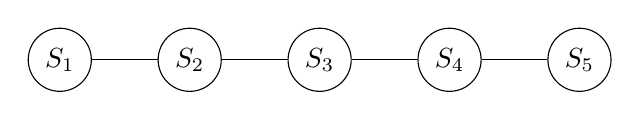
\begin{tikzpicture}[every node/.style={circle,draw,minimum size=8mm},node distance=1.65cm]
\node (s1) {$S_1$}; \node[right of=s1] (s2) {$S_2$}; \node[right of=s2] (s3) {$S_3$}; \node[right of=s3] (s4) {$S_4$}; \node[right of=s4] (s5) {$S_5$};
\draw (s1)--(s2)--(s3)--(s4)--(s5);
\end{tikzpicture}
\end{center}
Vecinatatile sunt
\[
N(S_1)=\{S_2\},\quad N(S_2)=\{S_1,S_3\},\quad
N(S_3)=\{S_2,S_4\},\quad N(S_4)=\{S_3,S_5\},\quad N(S_5)=\{S_4\}.
\]
Graful este conex si are $|V|=5$, $|E|=4=|V|-1$; deci este arbore si nu contine cicluri.

\section*{b) Factorii modelului Markov}
Construim un model Markov discret cu cate un factor unar pe fiecare nod:
\[
\phi_i(0)=0.5,\qquad \phi_i(1)=0.3,\qquad \phi_i(2)=0.2,\qquad i=1,\dots,5.
\]
Pentru fiecare muchie $(i,j)\in E$, atasam un factor de pereche
\[
\phi_{ij}(s_i,s_j)=\Psi_{s_i,s_j}.
\]
De exemplu, $\phi_{12}(0,0)=0.7$, $\phi_{23}(0,1)=0.2$, $\phi_{34}(1,2)=0.2$ si $\phi_{45}(2,2)=0.6$. In total avem $5$ factori unari si $4$ factori de pereche, adica $9$ factori. Acest model se poate construi in \texttt{pgmpy} cu \texttt{MarkovNetwork} si \texttt{DiscreteFactor}; codul si graful afisat programatic se includ in notebook.

\section*{c) Distributia comuna si normalizarea}
Definim ponderea nenormalizata a unei configuratii $s=(s_1,\ldots,s_5)$:
\begin{align*}
w(s)&=\prod_{i=1}^{5}\phi_i(s_i)\prod_{(i,j)\in E}\phi_{ij}(s_i,s_j)\\
&=p(s_1)p(s_2)p(s_3)p(s_4)p(s_5)\,\Psi_{s_1,s_2}\Psi_{s_2,s_3}\Psi_{s_3,s_4}\Psi_{s_4,s_5}.
\end{align*}
Distributia comuna este
\[
\boxed{P(s_1,\ldots,s_5)=\frac{w(s_1,\ldots,s_5)}{Z}},\qquad
\boxed{Z=\sum_{s_1=0}^{2}\cdots\sum_{s_5=0}^{2}w(s_1,\ldots,s_5)}.
\]
Exista $3^5=243$ configuratii. Ca exemplu, pentru $s=(0,0,1,2,2)$ avem
\begin{align*}
\prod_i p(s_i)&=0.5\cdot0.5\cdot0.3\cdot0.2\cdot0.2=0.003,\\
\prod_{(i,j)\in E}\Psi_{s_i,s_j}&=0.7\cdot0.2\cdot0.2\cdot0.6=0.0168,\\
w(0,0,1,2,2)&=0.003\cdot0.0168=0.0000504.
\end{align*}
Pentru a calcula $Z$ fara sa scriem manual 243 de produse, folosim matricea
\[
T_{ab}=\Psi_{ab}p(b),\qquad
T=\begin{pmatrix}
0.35&0.06&0.02\\
0.10&0.18&0.04\\
0.05&0.09&0.12
\end{pmatrix}.
\]
Cu $\mathbf{1}=(1,1,1)^{\mathsf T}$ si $p$ vector linie, suma tuturor configuratiilor este
\[
Z=pT^4\mathbf{1}=\boxed{0.020409725}.
\]
Prin urmare, pentru configuratia din exemplu,
\[
P(0,0,1,2,2)=\frac{0.0000504}{0.020409725}\approx\boxed{0.00246941}.
\]
Prin constructie, $\sum_s P(s)=Z/Z=1$.

\section*{d) Marginala unei statii neobservate}
Presupunem ca observam
\[
O=\{S_1=0\ (\mathrm{Soare}),\ S_5=2\ (\mathrm{Nori})\}.
\]
Statiile $S_2,S_3,S_4$ sunt necunoscute. Raman $3^3=27$ configuratii compatibile. Constanta pentru aceste configuratii este
\begin{align*}
Z_O&=\sum_{s_2,s_3,s_4=0}^{2}w(0,s_2,s_3,s_4,2)\\
&=\boxed{0.00111135}.
\end{align*}
Observatie: $Z_O$ este \emph{suma ponderilor compatibile}, nu $P(O)$; de fapt $P(O)=Z_O/Z$.

Cautam distributia conditionata a lui $S_3$:
\[
\boxed{P(S_3=k\mid O)=\frac{\displaystyle\sum_{s_2=0}^{2}\sum_{s_4=0}^{2}w(0,s_2,k,s_4,2)}{Z_O}},\qquad k\in\{0,1,2\}.
\]
De exemplu, pentru $k=0$ (Soare) fixam $S_3=0$ si adunam dupa toate cele 9 perechi $(s_2,s_4)$. Rezultatele sumelor sunt
\[
\begin{array}{c|ccc}
k &0\ (\mathrm{Soare})&1\ (\mathrm{Ploaie})&2\ (\mathrm{Nori})\\\hline
\displaystyle\sum_{s_2,s_4}w(0,s_2,k,s_4,2)
&0.00076405&0.00023520&0.00011210
\end{array}
\]
Verificare: $0.00076405+0.00023520+0.00011210=0.00111135=Z_O$. Normalizam fiecare valoare:
\begin{align*}
P(S_3=0\mid O)&=\frac{0.00076405}{0.00111135}\approx0.687497,\\
P(S_3=1\mid O)&=\frac{0.00023520}{0.00111135}\approx0.211634,\\
P(S_3=2\mid O)&=\frac{0.00011210}{0.00111135}\approx0.100868.
\end{align*}
Suma celor trei probabilitati este aproximativ $1$ (diferenta provine din rotunjire). Starea cu probabilitatea maxima este
\[
\boxed{\operatorname{MAP}_{\mathrm{marginal}}(S_3)=\arg\max_{k\in\{0,1,2\}}P(S_3=k\mid O)=0\ (\mathrm{Soare})}.
\]

\section*{e) MAP comun si comparatia cu maximele marginale}
Trebuie sa alegem \emph{simultan} cele trei stari necunoscute:
\[
(s_2^*,s_3^*,s_4^*)=\arg\max_{s_2,s_3,s_4}P(s_2,s_3,s_4\mid O).
\]
Deoarece $Z_O>0$ este acelasi pentru toate cele 27 de configuratii compatibile,
\[
(s_2^*,s_3^*,s_4^*)=\arg\max_{s_2,s_3,s_4}w(0,s_2,s_3,s_4,2).
\]
Maximul este atins pentru $(s_2,s_3,s_4)=(0,0,0)$. Calculul explicit al ponderii este
\begin{align*}
w(0,0,0,0,2)
&=(0.5^4\cdot0.2)(0.7^3\cdot0.1)\\
&=0.0125\cdot0.0343=\boxed{0.00042875}.
\end{align*}
Probabilitatea conditionata a acestei configuratii este
\[
P(S_2=0,S_3=0,S_4=0\mid O)=\frac{0.00042875}{0.00111135}\approx\boxed{0.385792}.
\]
Configuratia completa MAP este deci
\[
\boxed{(S_1,S_2,S_3,S_4,S_5)=(\mathrm{Soare},\mathrm{Soare},\mathrm{Soare},\mathrm{Soare},\mathrm{Nori})}.
\]
Pentru comparatie, marginalele celorlalte doua statii necunoscute (calculate prin aceeasi metoda de insumare) sunt:
\[
\begin{array}{c|ccc|c}
&\mathrm{Soare}&\mathrm{Ploaie}&\mathrm{Nori}&\mathrm{MAP\ marginal}\\\hline
S_2&0.842444&0.120394&0.037162&\mathrm{Soare}\\
S_3&0.687497&0.211634&0.100868&\mathrm{Soare}\\
S_4&0.443380&0.267782&0.288838&\mathrm{Soare}
\end{array}
\]
Asadar, in \emph{acest} exemplu, maximele marginale alese separat dau tot $(0,0,0)$ si coincid cu MAP comun. \textbf{Nu coincid intotdeauna.} Contraexemplu separat, pentru doua variabile binare $X,Y$:
\[
\begin{array}{c|cc}
 &Y=0&Y=1\\\hline
X=0&0.35&0.05\\
X=1&0.30&0.30
\end{array}
\]
Aici $P(X=1)=0.60$, iar $P(Y=0)=0.65$, deci maximele marginale formeaza $(1,0)$, cu probabilitatea $0.30$. Totusi MAP comun este $(0,0)$, cu probabilitatea $0.35$. Prin urmare, maximizarea fiecarei marginale separat nu este echivalenta, in general, cu maximizarea distributiei comune.

\section*{Concluzie}
Am ales un arbore cu 5 statii si am definit 5 factori unari si 4 factori de pereche. Am obtinut $Z=0.020409725$ prin insumarea ponderilor celor 243 de configuratii. Pentru observatiile $S_1=\mathrm{Soare}$ si $S_5=\mathrm{Nori}$, predictia marginala la $S_3$ este Soare, iar MAP comun este $(\mathrm{Soare},\mathrm{Soare},\mathrm{Soare},\mathrm{Soare},\mathrm{Nori})$. Codul \texttt{pgmpy} din notebook trebuie anexat pentru constructia si afisarea efectiva a grafului si factorilor.
\end{document}